\chapter{Context and Goals definitions}
\label{chap:context_and_goals}

\section{Context Definition}
\label{sec:context}
Maintenance is one of the most important tasks to assure the quality and correct operation of any kind of system. Even the highest quality systems, built by the best engineers to operate for long periods with the least possible human assistance, will eventually be exposed to damage or malfunction. In order to avoid the negative effects that system malfunction can produce, a significant amount of resources and effort is usually needed to be put on maintenance tasks. However, putting resources and effort on maintenance procedures might still not be enough if the procedures and strategies are not adequate and efficient.

Traditionally, we have discerned between two types of maintenance procedures:
\begin{itemize}
\item \emph{Corrective maintenance} is the most common approach, although it has very important limitations. With this approach, elements of our system are repaired or replaced once they have failed or worn out, to bring them back to operation. This usually means a high downtime in operation, as no actions are taken until our system is already malfunctioning.

\item \emph{Preventive maintenance} focuses on preventing these failures. Elements can be periodically examined and analysed in order to control their operation and perform simpler procedures to adjust them before reaching malfunction and downtime. This approach means much higher costs, as a significantly bigger amount of time is needed to monitor the elements on our system and correct them. However, as downtime means business losses in almost all cases, these higher costs usually pay back in terms of loss reduction.
\end{itemize}

A balance can be easily achieved by spending on preventive maintenance not more than the losses we would suffer from downtime if we were using a corrective approach.

However, the costs of preventive maintenance can be drastically reduced by optimising procedures and using the adequate techniques. For example, we can reduce the amount of variables and magnitudes we are monitoring (and which cost us money to monitor) if we know which ones give the better insight on the status on our systems. The same can be done with corrective maintenance. If we can somehow foresee which systems are going to fail, we can be prepared and reduce impact on our business even if we cannot do anything to prevent its failure.

In both cases, \emph{prediction} can be a key element for maintenance optimisation. Either we know which are the indicators of a system deterioration which we can repair, or we know which systems are going to fail and when to be prepared and optimise corrective procedures. We can even speak of a new type of maintenance - \emph{predictive maintenance} - which embraces several techniques to try and obtain this knowledge of future events.

\section{Project Objectives}
The project \emph{Trainmining} aims to design predictive maintenance techniques on already-existing maintenance stations of a railway network. These maintenance stations monitor different elements and subsystems over a railway line and raises alarms whenever a line element fails or requires human intervention. Additionally, maintenance workers perform different preventive maintenance procedures, gathering information about several parameters on each element and performing the appropriate actions when needed. Acquisition of values and determination of necessary actions is however not automatised within the maintenance stations, and workers have to manually perform these tasks.

In order to design \emph{predictive procedures} for the railway network, we have a big amount of event logs gathered by the maintenance stations, as well as registries filled by maintenance workers when performing preventive tasks. We will therefore try to extract, from that large amount of data, knowledge on how to predict future events from current observations

In this direction, \emph{Data Mining} techniques can be extremely useful in order to find relations between patterns in environment variables and the occurrence of events, or even relations between events themselves. These relations, which may at first not be apparent for the human mind, can be obtained through different automated learning processes, and thus infer markers which will act as indicators of when and how failures can happen. In order to extract this data we will need to count on a significantly high amount of event logs, gathered during previous years, on which we will apply said techniques.

First of all, we need to define the learning objectives of our project: what kind of information we aim to extract from all the available data. In latest terms, what we want is to be able to predict future events based on events from the past. A prediction will be based on one or more past events (the \emph{antecedent}) and indicate one or more events than are likely to happen in the future (the \emph{consequent}). Furthermore, we can impose restrictions in terms of time. For instance, we should limit the temporal distance between events in the antecedent, and estimate how far in the future the consequent will happen. Finally, as giving a certain prediction that will be true \emph{everytime}, our prediction will have an associated \emph{confidence}, which can be described as the probability for our prediction to be true. A graphic representation of a generic prediction can be seen in figure~\ref{fig:ass_rule}.

Table~\ref{tab:objectives_methods} contains a summary of learning objectives, along with the working methods which will be followed for each of them as is explained in section~\ref{sec:methods}.

\begin{figure}[hbtp]
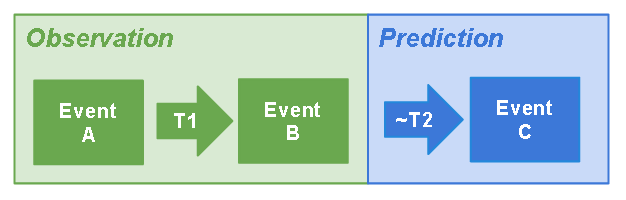
\includegraphics[width=\textwidth]{./img/association_rules.png}
\caption{A general prediction} \label{fig:ass_rule}
\end{figure}


The events forming the \emph{consequent} of our prediction will be alarms raised by the maintenance stations - we want to prevent or be prepared for the alarms happening in the future - and the antecedent can be formed by different kind of elements. In our case, both terms will be formed by system events. This means that we will predict future events taking as evidence other events which have already happened.

This working line consists of acquiring knowledge on how events are related to each other in terms of occurrence. In other terms, the events in the antecedent of our predictions will be formed by alarms (as well as the consequent, as we said before). Among all the alarms raised on the maintenance stations, some of them may be directly triggered by previous ones, having a direct occurrence relation; or might be caused by the same environmental conditions, being most likely for them to happen along the same time periods. As a result, even in cases where they might seem completely unrelated, the occurrence of one of them can give us information on the chances of others happening within a defined time span.

Our objective is to find and analyse these relations and use them to build useful predictions. Depending on the parameters we use for our knowledge discovery procedures, we might obtain different types of rules. For instance, varying the temporal resolution of our analysis, we might obtain rules to predict events in terms of months, days or hours. Depending on the timespan we work with, our prediction rules may be useful to prevent failures, to be prepared to fix them, or be completely useless if there is not enough anticipation.

It is important to note that in the railway network we are working with, there are different maintenance stations in different railway lines. Neither the maintenance stations or the lines are equal throughout the whole network, and therefore we may have to follow different procedures and expect different results for each of them. Initially, we will treat every station (along with the set of elements under its management) independently, even though we already know their classification and the similarities between them. Unless generalisation is evident and clearly convenient, we will always maintain this separation and obtain a different set of rules for each of them.

Due to the characteristics and large size of the available data, we are likely to find a vast amount of frequent sequences and association rules from which not all of them will be useful for maintenance purposes. Different metrics can be applied to evaluate the \emph{importance} of a rule, such as its confidence (its probability to be true on a given situation), the severity of the predicted events, or its support (absolute frequency of the sequence happening).

A comprehensive analysis is necessary to extract the most useful association rules from the set and discard the others, in order to obtain the most efficient set possible. Additionally, the different metrics can even allow predictions to be filtered in real time, according to the available resources or the desired results.

In figure~\ref{fig:demo_view} we can view an example use case. A maintenance operator could view the alarms which are being raised by the maintenance station (in a similar way as the current systems) and a list of predicted alarms - along with the confidence of the prediction and an estimated time span - based on those past and current alarms.

\begin{figure}[hbtp]
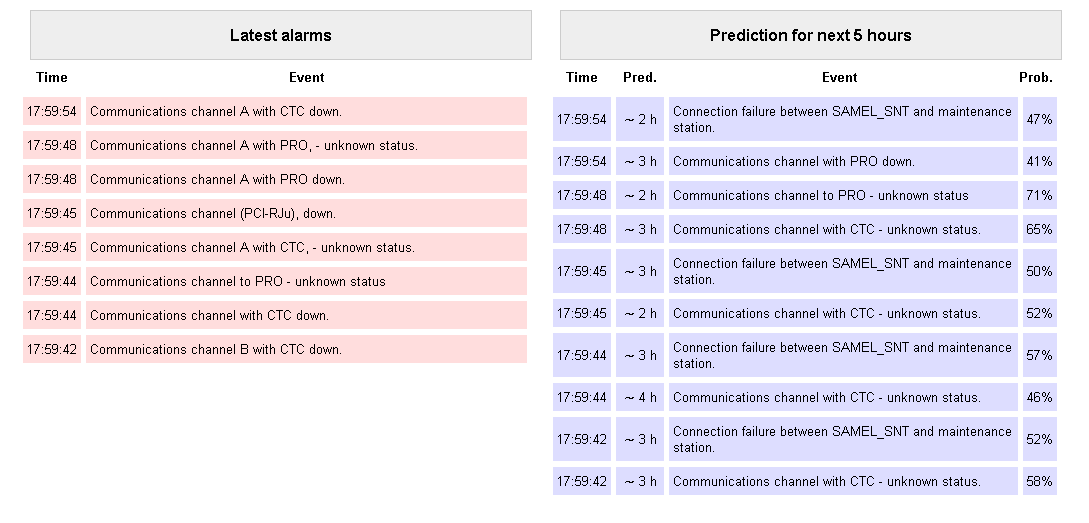
\includegraphics[width=\textwidth]{img/demo_thales.png}
\caption{An example use case} \label{fig:demo_view}
\end{figure}

\section{Data Description}
For this project, Thales Group, a leader company in the development of railway systems in Spain is cooperating with the research group {\it Grupo de Sistemas Inteligentes} from the Universidad Politécnica de Madrid, with large expertise in the application of intelligent systems to real problems. Thales Spain has developed an advanced system called \emph{maintenance station}, which diagnoses, gathers and visualises different kind of events happening along the railway network. These maintenance stations comprise different advanced diagnosis systems, which can identify and report several kind of events happening along the lines which might require human intervention. These stations gather logs with all the events which have happened in the past, which will allow us to study and analyse the operation of these stations during the past.

At the moment of writing this document, we count on data of three maintenance stations (B, C and D), which are located in Spain. Each of these stations controls a different railway line, and have different diagnosis systems and characteristics, as shown in table~\ref{tab:stations}. In this table we see that the three lines we are working with are of different types and have different diagnosis systems. Specifically, Stations B and C control high speed lines, while Station D controls a commuter line. Different types of lines will have different elements and systems, and results are therefore expected to be different in both groups. Furthermore, supervised systems are different in all the three stations, which means that alarms received from each of them will not necessarily be the same. Details on number of events and time span of the available data is given on table~\ref{tab:data_details}.

\begin{table}
\begin{center}
\begin{tabular}{|c|c|c|}
\hline \headcell{Name} & \headcell{Line type} & \headcell{Supervised systems} \\ 
\hline
\hline Station B & High Speed & SAM-E-L \\ 
\hline Station C & High Speed & ERTMS (levels 1 and 2) \\ 
\hline Station D & Commuter & Diagnosis and Energy \\ 
\hline 
\end{tabular}
\\
\bigskip
ERMTS: European Rail Traffic Management System\\
SAM-E-L: Sistema de Ayuda al Mantenimiento para Ence (Local)\\

\end{center} 
\caption {Maintenance Stations} \label{tab:stations} 
\end{table}

\begin{table}
\begin{center}
\begin{tabular}{|c|c|c|c|c|}
\hline \headcell{Station} & \headcell{N. of events} & \headcell{Start date} & \headcell{End date} & \headcell{Period} \\ 
\hline
\hline Station B & 185274 & 18-01-2010 & 31-05-2010 &  5 months \\ 
\hline Station C & 304408 & 30-11-2007 & 03-06-2009 &  1.5 years \\ 
\hline Station D & 118026 & 17-05-2011 & 09-04-2012 &  1 year \\ 
\hline 
\end{tabular}
\end{center} 
\caption {Available data} \label{tab:data_details} 
\end{table}

\subsection{Database description}
\label{sec:database_description}
In order to properly process the data provided in form of database backups, it is of essential importance that we completely understand how data is represented in databases. We will analyse the structure and how data is represented in the provided databases (one for each station). Each of these databases corresponds to a single \emph{maintenance station}, which comprises a whole railway line with several elements along it. The elements with diagnosis systems which can raise alarms are called \emph{installations}, and have different sets of sensors and other systems to control \emph{field elements}. An schematic representation of this architecture is represented in figure~\ref{fig:arch_stations}. The detailed description of available systems and subsystems is of few interest to us. Initially we will only need to differentiate between maintenance stations and installations.

\begin{figure}[hbt]
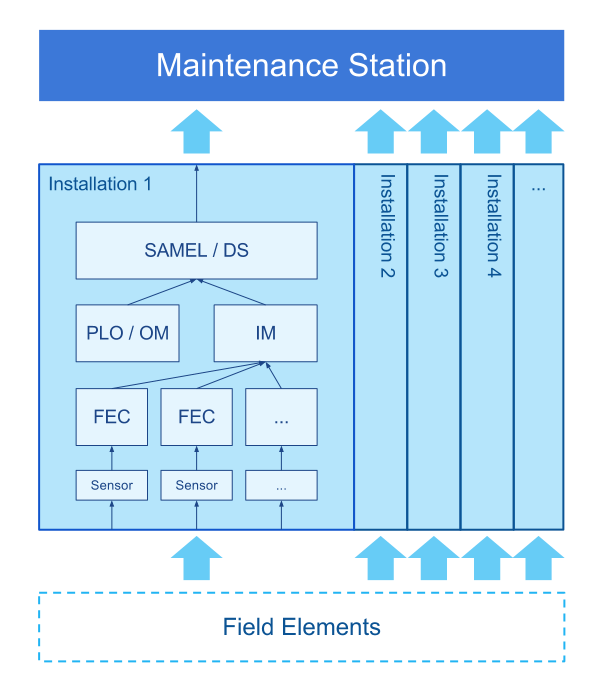
\includegraphics[width=\textwidth]{./img/arch_stations.png}
\caption{Simplified diagram of the maintenance systems architecture} \label{fig:arch_stations}
\end{figure}

Each \emph{maintenance station} has its own unique database, which is of great convenience in order to treat different stations independently. We will start analysing the structure of the main tables of said databases. Due to the high complexity of the maintenance stations, there are a vast amount of tables with configuration parameters and other operational values which are not of interest for our purposes. With assistance from Thales engineers, we have reduced the tables only to those which characterise registered alarms. A total of 4 different tables is used in order to register this information, which are the following:

\begin{description}
\item[Table ER\_ERRORS] This table contains an entry for every alarm received by the maintenance station. Its fields are detailed on table~\ref{tab:table_er_errors}.
\item[Table IG\_INSTALLATIONGENERAL] This table contains information on all the installations managed by the maintenance station. Its fields are detailed on table~\ref{tab:table_ig_installationgeneral}
\item[Table IG\_NODO\_INSTALLATION] This table gathers additional information on installations which are nodes. Nodes are installations which can raise alarms but need a parent installation to send them to the maintenance station. Its fields are detailed on table~\ref{tab:table_ig_nodo_installation}
\item[ERS\_ERRORS\_SAM\_ENCE] This table contains detailed information about the alarms. Its fields are detailed on table~\ref{tab:table_ers_errors_sam_ence}
\item[ERH\_ERRORS\_HSL1] This table is equivalent to ERS\_ERRORS\_SAM\_ENCE. Maintenance stations use one or the other depending on how they receive the alarms. Its only difference with ERS\_ERRORS\_SAM\_ENCE is that registers the method used to receive the alarm. For our purposes it will be treated exactly as its equivalent, and therefore its structure can also be reviewed in table~\ref{tab:table_ers_errors_sam_ence}
\end{description}

Concluding, for each alarm we will have a timestamp and an alarm identifier in table ER\_ERRORS. Alarm identifier is a foreign key which points to table ERS\_ERRORS\_SAM\_ENCE (or equivalent) in which further details of the alarm are saved. Among these details, we can find an installation identifier which specifies which installation has produced the alarm. That identifier is also a foreign key pointing to table DVNI\_INSTALLATIONCODE, in which further details about the installation are stored. Further details on all the database fields are given in tables~\ref{tab:table_er_errors}, \ref{tab:table_ig_installationgeneral}, \ref{tab:table_ig_nodo_installation} and \ref{tab:table_ers_errors_sam_ence}.


\begin{table}
\begin{tabularx}{\textwidth}{|l|X|}
 \hline \headcell{Field name} & \headcell{Description} \\
 \hline
 \hline DVNI\_ERRORNUMBER & Alarm identifier \\
 \hline DVNS\_ERRORTIME & Time-stamp for the alarm \\
 \hline DVNI\_INSTALLATIONCODE & Code of the installation in which the alarm was raised \\
 \hline DVNI\_SENDERINSTALLATIONCODE & Code of the installation from which the alarm was sent (might be different from the one which raised it) \\
 \hline
\end{tabularx}
\caption{Detail of fields on table ER\_ERRORS} \label{tab:table_er_errors}
\end{table}

\begin{table}
\begin{tabularx}{\textwidth}{|l|X|}
 \hline \headcell{Field name} & \headcell{Description} \\
 \hline
 \hline DVNI\_INSTALLATIONCODE & Installation identifier  \\
 \hline DVNI\_SYSTEMCODE & Type of system, as defined in the ``SG\_SYSTEMSGENERAL'' table \\ 
 \hline DVNI\_VERSION & System version \\
 \hline DVAC\_SHORTNAME & Short name of the installation \\
 \hline DVAC\_INSTALLATIONNAME & Name of the installation \\
 \hline DVAC\_LOCATION & Location for the installation \\
 \hline CHK\_IS\_NODE & Whether it is a node (doesn't directly send alarms, only raise them) or not \\
 \hline
\end{tabularx}
\caption{Detail of fields on table IG\_INSTALLATIONGENERAL} \label{tab:table_ig_installationgeneral}
\end{table}

\begin{table}
\begin{tabularx}{\textwidth}{|l|X|}
 \hline \headcell{Field name} & \headcell{Description} \\
 \hline
 \hline IG\_NODO\_INSTALLATION & Identifier of the installation which is a node \\
 \hline DVNI\_FATHER\_INSTALLATION & Identifier of the parent installation \\
 \hline
\end{tabularx}
\caption{Detail of fields on table IG\_NODO\_INSTALLATION} \label{tab:table_ig_nodo_installation}
\end{table}

\begin{table}
\begin{tabularx}{\textwidth}{|l|X|}
 \hline \headcell{Field name} & \headcell{Description} \\
 \hline
 \hline DVNI\_ERRORNUMBER & Alarm identifier \\
 \hline MESSAGE\_ID & Unique alarm identifier \\
 \hline MESSAGE\_TYPE & Type of alarm, always set as ``notification'' (not relevant) \\
 \hline INVOKE\_TYPE & Tells whether the alarm has generated itself due to a connection or disconnection (if type is ``node'') or is generated by a diagnosis system (``saml'') or energy system (``energy'') \\
 \hline INVOKE\_NAME & Irrelevant, always set to ``diagnosis'' \\
 \hline EVENT\_TYPE & Defines the type of alarm which has been generated. Its possible values are listed in table~\ref{tab:field_event_type}. \\
 \hline ADDITIONAL\_TEXT & Alarm code \\
 \hline ADDITIONAL\_INFOS & Additional parameters to be shown in error message \\
 \hline DVNI\_ERRORCATEGORY & Alarm severity. Values from 1 to 5 indicating importance of the alarm, or -1 if the alarm indicates recovery from a previous failure. \\
 \hline
\end{tabularx}
\caption{Detail of fields on table ERS\_ERRORS\_SAM\_ENCE} \label{tab:table_ers_errors_sam_ence}
\end{table}

\begin{table}
\begin{tabularx}{\textwidth}{|l|X|}
  \hline \headcell{Event type} & \headcell{Description} \\
  \hline
  \hline fieldElementAlarm & Alarm related to a field element \\
  \hline fieldElementFailure & Failure in a field element \\
  \hline operatorInformation & Information to the operator \\
  \hline imCpuAndCommunications & Related to IM CPU or IM communications \\
  \hline internalDiagnosis & Internal diagnosis of a system \\
  \hline operationsDiagnosisCommunications & Communication error in Operation and Diagnosis systems \\
  \hline ImFecVersions & IM or FEC version \\
  \hline internalTraces & Internal traces of a system \\
  \hline operatorCommandAnswer & Answer to an operator command \\
  \hline CommProblem & Undefined communication problem \\
  \hline Information & Information message: versions, etc. \\
  \hline CommunicationsAlarm & Procedures and processes to carry information from one point to other \\
  \hline QualityOfServiceAlarm & Loss of quality of service \\
  \hline ProcessingErrorAlarm & SW or processing error \\
  \hline EquipmentAlarm & Equipment failure \\
  \hline EnvironmentAlarm & Related to the environment where the system is located \\
  \hline other & Other \\
  \hline
\end{tabularx}
\caption{Description of values for the field EVENT\_TYPE} \label{tab:field_event_type}
\end{table}
\clearpage

\subsubsection{Reduced representation of alarms}
\label{sec:reduced_alarms}
In section~\ref{sec:database_description} we have seen a deep definition of all the tables characterising registered alarms. Each of these tables contain several fields, which in total makes an inconvenient large number of variables. While all of them are necessary for correct system function and maintenance purposes, not all of them will be necessary for us to work with alarms.

In order to characterise an event, the main things we need to know can be reduced to three variables:
\begin{itemize}
\item What has happened
\item When has it happened
\item Where has it happened
\end{itemize}

In section~\ref{sec:database_description} we have seen other variables which can provide additional information which - although not essential - can be useful. Specifically, we think the following data can be of possible interest:

\begin{itemize}
\item How severe the event is (severity)
\item Which type of event has happened (event type)
\end{itemize}

These variables can help us to classify alarms or give more importance to those which are more severe. As this information is already provided on given databases, we will keep it and use it for better alarm classification and filtering. However, none of them are essential in order to characterise alarms, as both of them give information which is already implicit in our previous \emph{``what has happened''} variable. Specifically, this information will be of great help in order to make a preliminary statistical insight on the events of the databases, for which a generalisation in terms of severity and category can help us have a better overview of the situation.

We have to identify which fields on our database corresponds to each of the variables we want to obtain. A direct relation is not possible, as details on \emph{what} has happened is registered in several fields of the database. This is necessary for maintenance purposes and better alarm handling in the maintenance station, but for our purposes we should identify \emph{what} has happened with a single variable.

In our database, we have unique alarm identifiers for each of the alarms. For better handling and understanding of what is happening, we will use the textual identifier of the events to identify them. This identifier is gathered on the \emph{ADDITIONAL\_TEXT} field, and can be translated to a full comprehensive human-readable message by the maintenance station. Furthermore, there is additional data to fill in details about the message. For example, we can have an alarm such as ``Communication channel with \emph{X} down'', being \emph{X} an additional parameter saved in the \emph{ADDITIONAL\_INFOS} field. Here we can follow two different approaches: disregard the information about \emph{X}, and just treat it as a ``Channel down'' error; or easily build a compact representation including both variables, such as ``channel.down/x''.

\subsection{Data preprocessing}
As we already mentioned, most data mining processes are usually focused on predicting the value of some variables given the value of the rest variables in a given observation. They work with discrete observations for which each of the variables is analysed or predicted. In our databases we have continuous observations, which need to be transformed into discrete observations\cite{zaki2001spade}.

Depending on the specific application we are using, we can need to transform this data into two possible formats. The first one is the called \emph{basket format}. The most typical example usually used to explain it is a registry of clients of a shop which keeps lists of what the clients buy (hence the name). Therefore, for each observation (often called \emph{transactions} again as an analogy to clients buying in a shop) we will have a list of items happening during that observation (or bought in that transaction). It is important to note that we will keep the same number of variables as in our original data, only that we will stack several items in single entries to obtain discrete observations. It is also important to be careful with which variables we are stacking. While we need to combine all the alarms happening during the same period, it is important not to lose or combine the Installation value. As a result, time identifiers won't be unique in the whole transformed database, but the pair time 
identifier-installation identifier will.

An example can be seen in tables \ref{tab:data_before_discret} and \ref{tab:basket_example}. Table~\ref{tab:data_before_discret} is an example of the original data, and table~\ref{tab:basket_example} is the equivalent data transformed into basket format.

The second possible transformation is to represent the occurrence of each alarm with an additional variable. This means that we will need as many variables as the total number of possible different alarms in our system. Same as before, we must be careful to preserve data on installations, and create independent observations for each time slot and each installation. Each additional variable can represent the alarms in different ways. Either in a boolean sense (whether the alarms happens at least once or not at all) or the specific number of times the alarm has happened. In order not to lose information at this stage of processing, we will keep the specific amount of times each alarm has happened, which can be easily reduced to a boolean variable if appropriate for the application.

This second case is indeed a more strict representation of the \emph{basket format}. While in basket format we just needed a single variable where we could add all the alarms in the form of a list, here we need to specify exactly the number of times all the variables have happened. Both of them are equivalent and we can easily convert data from one format to another, but as different algorithms will work specifically with one of each forms of representation, it's convenient to perform both transformations from original data and use each one accordingly.

An example of this transformation can be seen in tables \ref{tab:data_before_discret} and \ref{tab:expanded_example}. Table~\ref{tab:data_before_discret} is an example of the original data, and table~\ref{tab:expanded_example} is the equivalent data discretised with additional variables.

These transformations have been automatised with R scripts, in a way so we can easily repeat these processes for different time spans. This will allow us to work at any moment with different time resolutions without any significant additional work for further transformations.

\begin{table}
\begin{center}
\begin{tabular}{|c|c|c|}
\hline \headcell{Timestamp} & \headcell{Installation} & \headcell{Alarm} \\ 
\hline
\hline 01-01-2011 00:00 & 0 & Alarm A \\ 
\hline 01-01-2011 00:30 & 0 & Alarm B \\ 
\hline 01-01-2011 00:45 & 1 & Alarm B \\ 
\hline 01-01-2011 01:10 & 0 & Alarm C \\ 
\hline 01-01-2011 01:20 & 0 & Alarm A \\ 
\hline 01-01-2011 01:22 & 0 & Alarm A \\
\hline 01-01-2011 01:25 & 1 & Alarm C \\ 
\hline 01-01-2011 01:30 & 1 & Alarm A \\ 
\hline 01-01-2011 02:20 & 0 & Alarm A \\ 
\hline 01-01-2011 02:30 & 1 & Alarm A \\ 
\hline 01-01-2011 02:45 & 0 & Alarm B \\ 
\hline ... & ... & ... \\ 
\hline 
\end{tabular} 
\end{center} 
\caption {Continuous observation. Example of alarms in log format.} \label{tab:data_before_discret} 
\end{table}

\begin{table}
\begin{center}
\begin{tabular}{|c|c|c|}
\hline \headcell{Time} & \headcell{Installation} & \headcell{Alarms} \\ 
\hline
\hline 0 & 0 & A, B \\ 
\hline 0 & 1 & B \\ 
\hline 1 & 0 & C, A, A \\ 
\hline 1 & 1 & C, A \\ 
\hline 2 & 0 & A, B \\ 
\hline 2 & 1 & A \\ 
\hline ... & ... & ... \\ 
\hline 
\end{tabular} 
\end{center}
\caption{An example of discretised data in basket format.} \label{tab:basket_example}
\end{table}

\begin{table}
\begin{center}
\begin{tabular}{|c|c|c|c|c|}
\hline \headcell{Time} & \headcell{Installation} & \headcell{Alarm A} & \headcell{Alarm B} & \headcell{Alarm C} \\ 
\hline 
\hline 0 & 0 & 1 & 1 & 0 \\ 
\hline 0 & 1 & 0 & 1 & 0 \\ 
\hline 1 & 0 & 2 & 0 & 1 \\ 
\hline 1 & 1 & 1 & 0 & 1 \\ 
\hline 2 & 0 & 1 & 1 & 0 \\ 
\hline 2 & 1 & 1 & 0 & 0 \\ 
\hline ... & ... & ... & ... & ... \\ 
\hline 
\end{tabular} 
\end{center} 
\caption {Example of discretised data} \label{tab:expanded_example} 
\end{table}

\clearpage


\section{Data Analysis}
In order to obtain a first general insight of what has happened during the time comprised by our backup data, we will perform a high-level preliminary statistic analysis. In order to achieve a qualitative idea of the type of events, we will use the additional variables we mentioned in section~\ref{sec:reduced_alarms}: severity and event type. These variables provide an already given alarm classification of interest for maintenance operators.

For this purpose, the R language provides a large amount of useful tools which can handle large amounts of data in a very efficient way\cite{quick2010statistical}.

\subsection{Event type distribution}
The first analysis we will perform consists on checking which event types appear in each maintenance station, and which percentage of the total amount of alarms corresponds to each of them. This will help us understand the nature of the events which are usually happening on our railway line.

First of all we will obtain a list of all the types found in each of the stations. We already described in table~\ref{tab:field_event_type} all the possible values for this field, but depending on the diagnosis systems installed on each of the stations, a different subset of them will be used. The list of events for each of the stations is given in tables \ref{tab:field_event_type_antequera} (Station B), \ref{tab:field_event_type_sevilla} (Station D) and \ref{tab:field_event_type_segovia} (Station C).

\begin{table}
\begin{tabularx}{\textwidth}{|l|X|}
  \hline \headcell{Event type} & \headcell{Description} \\
  \hline
  \hline fieldElementAlarm & Alarm related to a field element \\
  \hline fieldElementFailure & Failure in a field element \\
  \hline operatorInformation & Information to the operator \\
  \hline imCpuAndCommunications & Related to IM CPU or IM communications \\
  \hline internalDiagnosis & Internal diagnosis of a system \\
  \hline operationsDiagnosisCommunications & Communication error in Operation and Diagnosis systems \\
  \hline CommunicationsAlarm & Procedures and processes to carry information from one point to other \\
  \hline
\end{tabularx}
\caption{Event types found in Station A} \label{tab:field_event_type_antequera}
\end{table}

\begin{table}
\begin{tabularx}{\textwidth}{|l|X|}
  \hline \headcell{Event type} & \headcell{Description} \\
  \hline
  \hline fieldElementAlarm & Alarm related to a field element \\
  \hline fieldElementFailure & Failure in a field element \\
  \hline operatorInformation & Information to the operator \\
  \hline imCpuAndCommunications & Related to IM CPU or IM communications \\
  \hline internalDiagnosis & Internal diagnosis of a system \\
  \hline operationsDiagnosisCommunications & Communication error in Operation and Diagnosis systems \\
  \hline CommunicationsAlarm & Procedures and processes to carry information from one point to other \\
  \hline Other & other \\
  \hline
\end{tabularx}
\caption{Event types found in Station D} \label{tab:field_event_type_sevilla}
\end{table}


\begin{table}
\begin{tabularx}{\textwidth}{|l|X|}
  \hline \headcell{Event type} & \headcell{Description} \\
  \hline
  \hline CommProblem & Undefined communication problem \\
  \hline Information & Information message: versions, etc. \\
  \hline CommunicationsAlarm & Procedures and processes to carry information from one point to other \\
  \hline ProcessingErrorAlarm & SW or processing error \\
  \hline EquipmentAlarm & Equipment failure \\
  \hline EnvironmentAlarm & Related to the environment where the system is located \\
  \hline
\end{tabularx}
\caption{Event types found in Station C} \label{tab:field_event_type_segovia}
\end{table}

From these tables we can observe that alarm types in Stations B and D are the same (except for unclassified alarms in Station D marked as ``other''). From this we can infer that diagnosis systems in these two stations are the same or very similar, as confirmed by Thales' engineers. Station C however presents a different - although also expectedly similar - set of alarm categories. This is an indicator of diagnosis systems being very different in Station C than in the other two stations, as confirmed by Thales' engineers.

For better overview of distribution of these alarm types, we will create charts of their respective percentages for each of the stations. These charts can be seen in figures \ref{fig:antequera_chart} (Station B), \ref{fig:segovia_chart} (Station C) and \ref{fig:sevilla_chart} (Station D).

\begin{figure}[htb]
 \centering
 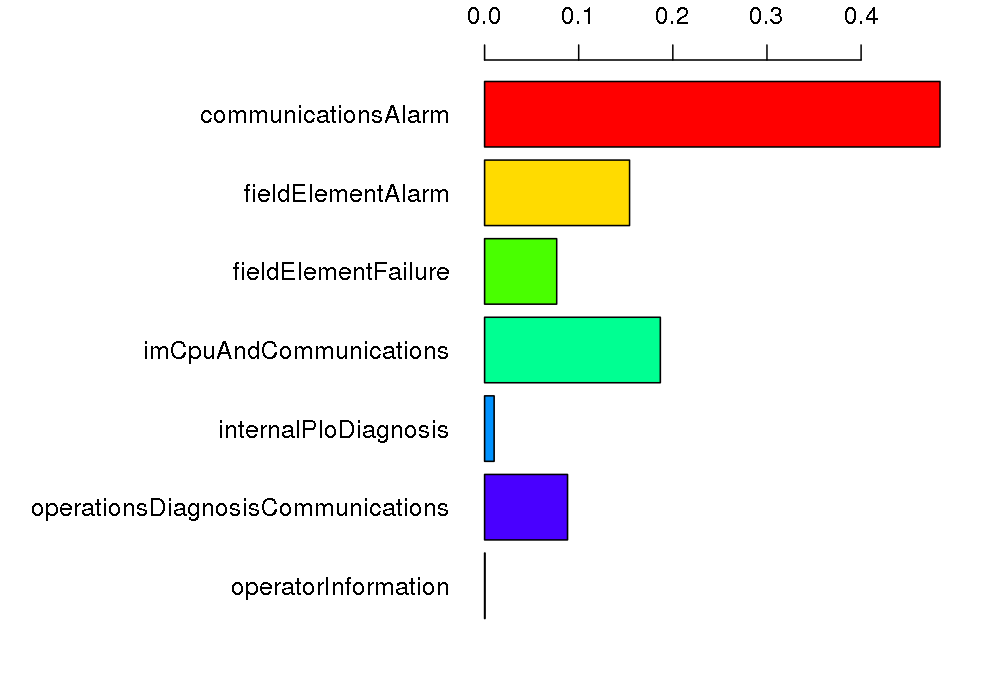
\includegraphics[width=\textwidth]{./img/antequera_graph.png}
 \caption{Alarm information for Station B}
 \label{fig:antequera_chart}
\end{figure}
\begin{figure}[htb]
 \centering
 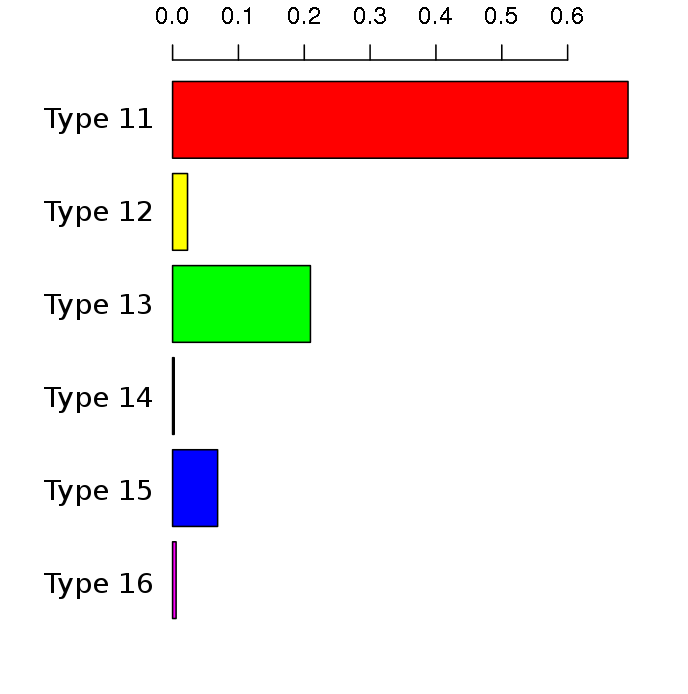
\includegraphics[width=\textwidth]{./img/segovia_graph.png}
 \caption{Alarm information for Station C}
 \label{fig:segovia_chart}
\end{figure}
\begin{figure}[htb]
 \centering
 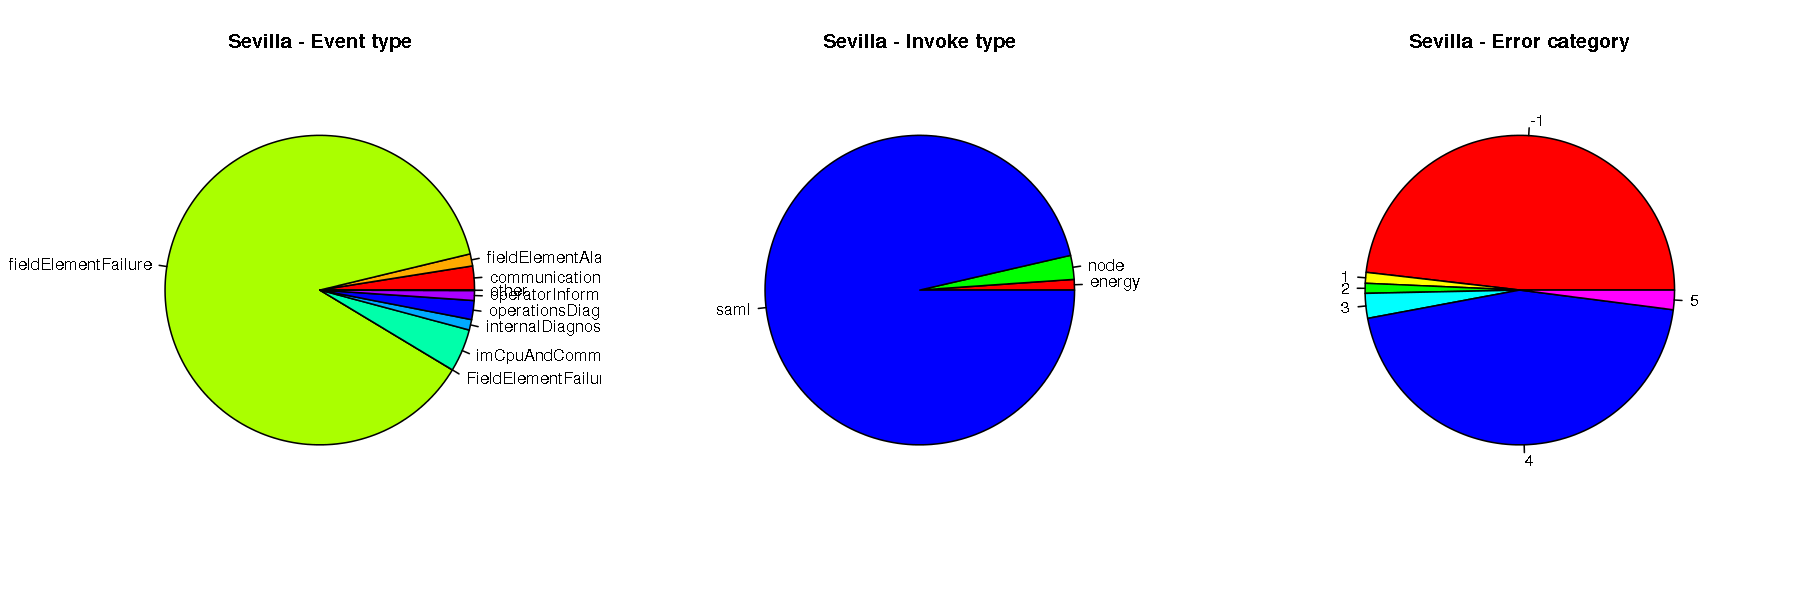
\includegraphics[width=\textwidth]{./img/sevilla_graph.png}
 \caption{Alarm information for Station D}
 \label{fig:sevilla_chart}
\end{figure}

\clearpage

We can see that in all of the stations, a single alarm type predominates among all of them. Specifically, we have a vast majority of communication alarms in Stations B and C, and a majority of field element failure alarms in Station D. This is not surprising due to the considerable differences between all of them, but can become a problem as the other categories may be too small compared to these main ones when performing Data Mining techniques, obtaining less information - or none at all - from them.

In this direction, it is possible that further actions are required in order to compensate these differences, and avoid that more frequent alarms overshadow the less frequent ones.

\subsection{Daily correlation}
In order to find further differences or similarities between the different stations, we will observe how alarm types are correlated to each others\cite{edwards1976introduction}. That is, how frequent is to find alarms of two specific types happening together during the same short period. For a first insight, we will analyse correlation during daily observations. This correlation information will not be of immediate help in order to predict alarms, as predicting the most frequent alarm type given some conditions is of very little - if any - help. However, it will give us a first idea on how strongly alarms are related to each others.

The result of this correlation is represented in figures \ref{fig:anteq_corr} (Station B), \ref{fig:segovia_corr} (Station C) and \ref{fig:sevilla_corr} (Station D).

\begin{figure}[htb]
 \centering
 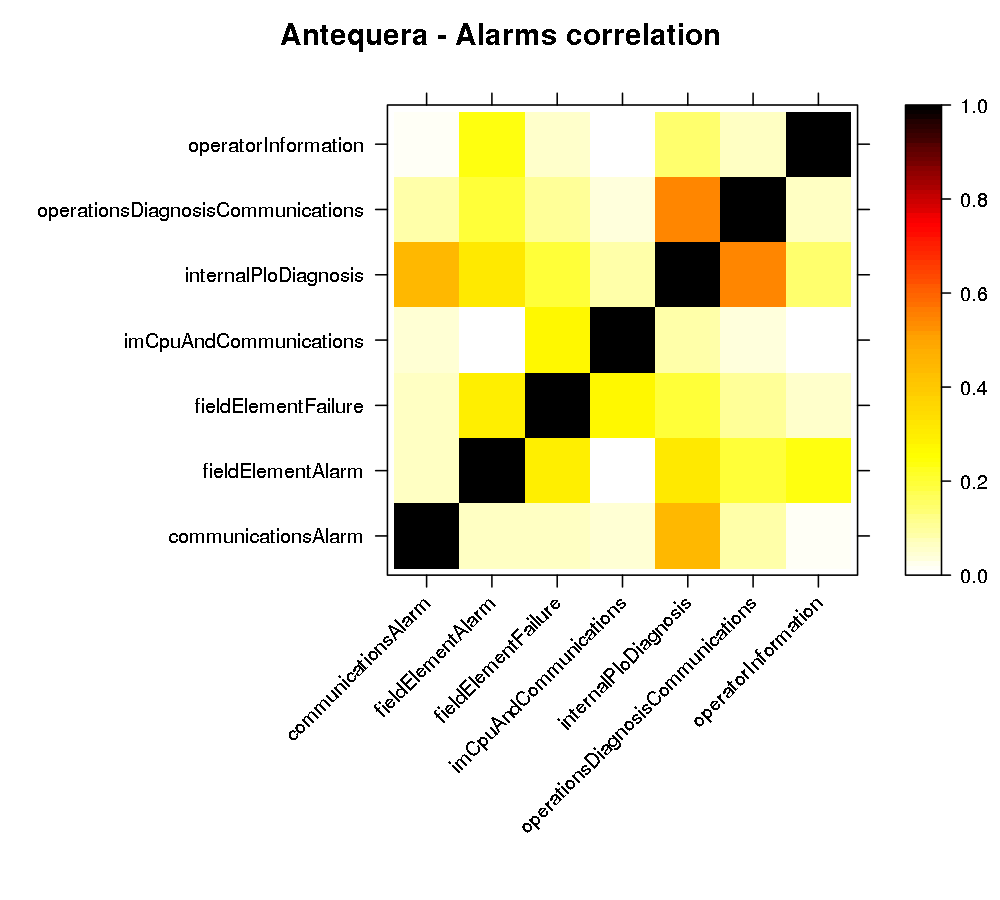
\includegraphics[width=\textwidth]{./img/antequera_corr.png}
 \caption{Daily correlation for Station B} \label{fig:anteq_corr}
\end{figure}
\begin{figure}[htb]
 \centering
 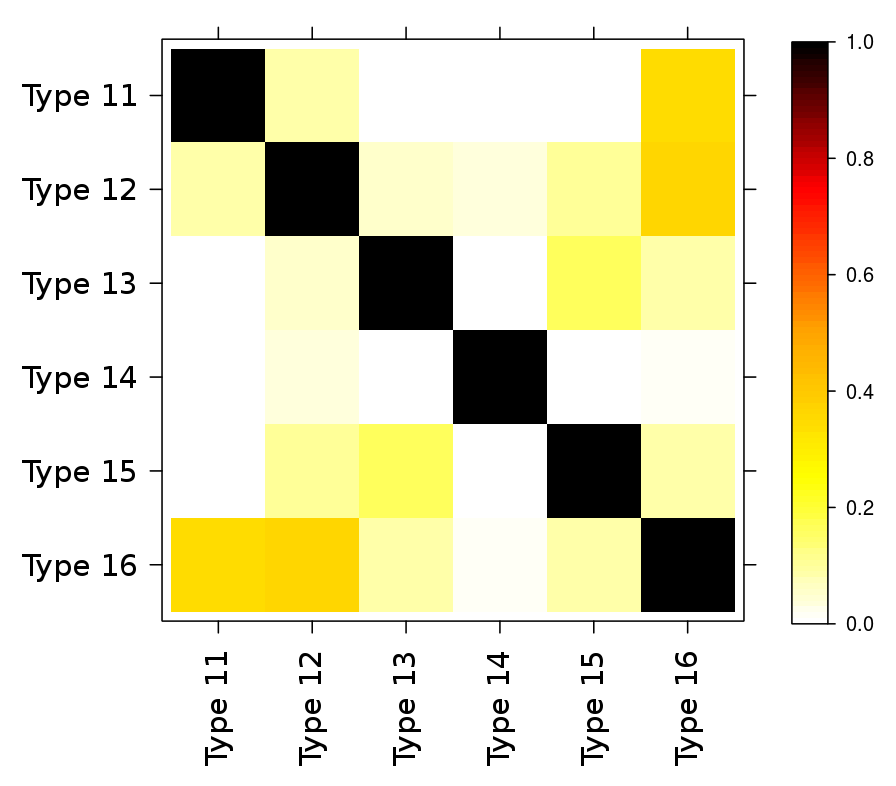
\includegraphics[width=\textwidth]{./img/segovia_corr.png}
 \caption{Daily correlation for Station C} \label{fig:segovia_corr}
\end{figure}
\begin{figure}[htb]
 \centering
 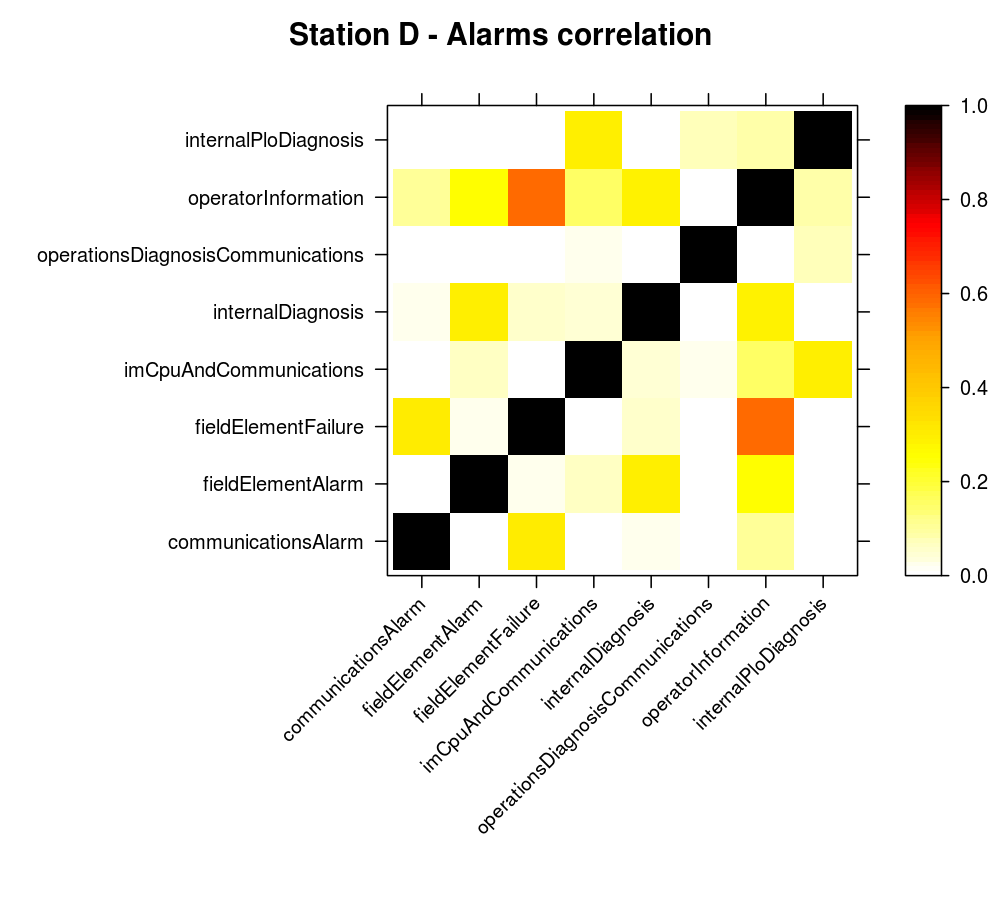
\includegraphics[width=\textwidth]{./img/sevilla_corr.png}
 \caption{Daily correlation for Station D} \label{fig:sevilla_corr}
\end{figure}

\clearpage

At first sight, we can affirm that these relations are different even in stations B and D, which we found to have similar diagnosis systems. This indicates that, even with similar diagnosis systems, the systems conforming both lines are different. This is indeed confirmed by Thales' engineers, as Station B controls a high speed line, while Station D corresponds to a commuter line.

Furthermore, we can see strong correlations in Station D (Field element failure and operator information) and Station C (Communications alarms and processing error alarms). As we don't have deep information of the nature of these categories, we can't affirm that this high correlation is due to any causal relation. However, we observe that both these cases show high correlation for the type of alarm which is more frequent in each station, so uneven distribution of alarms might be the cause of this apparent relation between alarms.

From this analysis we can conclude the significant differences in alarm relations between stations, confirming our first thoughts of impossibility of reducing the problem by generalising and merging data from different stations. Further analysis using specific alarm identifiers instead of categories will be needed to obtain relevant results.

\subsection{Hourly timeline}
As an additional first analysis, we wanted to overview the variation of alarm occurrence during the day. During a day, high differences in environment can be experimented which can affect systems in different ways. For instance, temperatures or train affluence can be very different from 4:00 AM to 1:00 PM. These differences can also be found during higher periods, for instance between weekdays and weekends, or between summer time and winter. To start with a specific observation period, we will perform a first analysis between day hours, leaving the other cases for future stages if considered adequate.

Charts with this analysis can be seen in figures \ref{fig:antequera_timeline} (Station B), \ref{fig:segovia_timeline} (Station C) and \ref{fig:sevilla_timeline} (Station D).

\begin{figure}[htb]
 \centering
 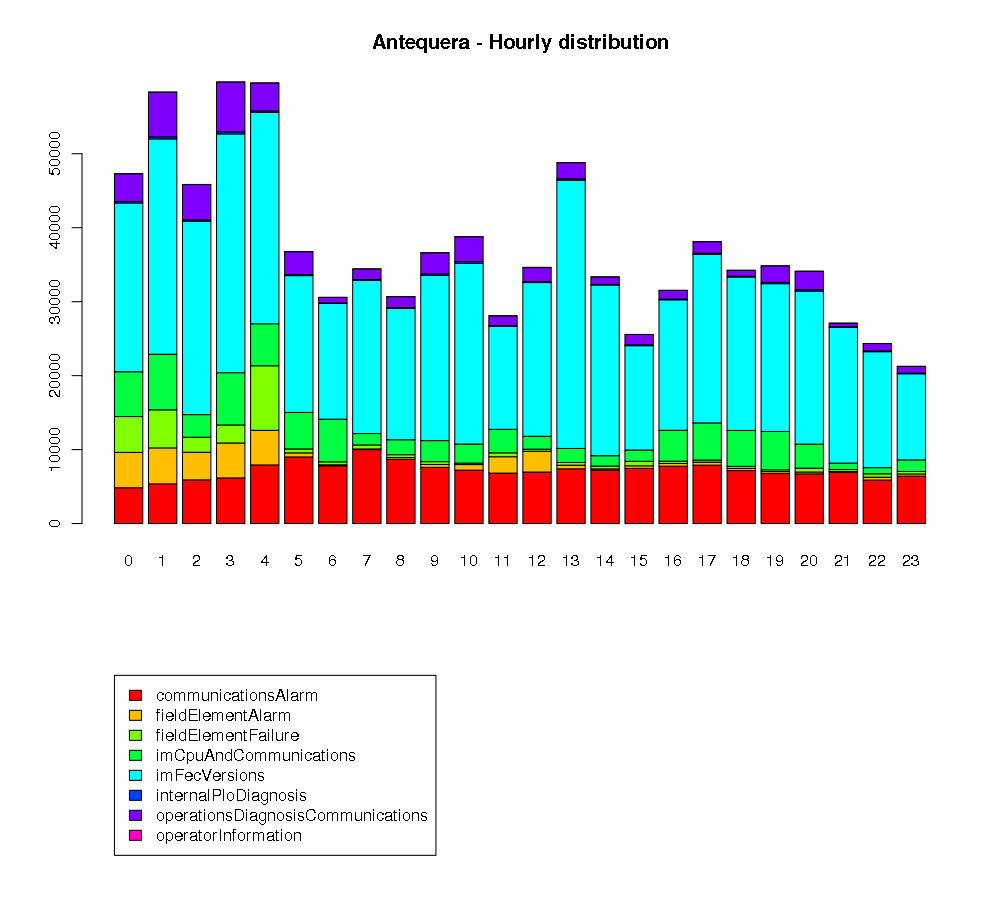
\includegraphics[width=\textwidth]{./img/antequera_timeline.png}
 \caption{Hourly distribution for Station B (stacked)} \label{fig:antequera_timeline}
\end{figure}
\begin{figure}[htb]
 \centering
 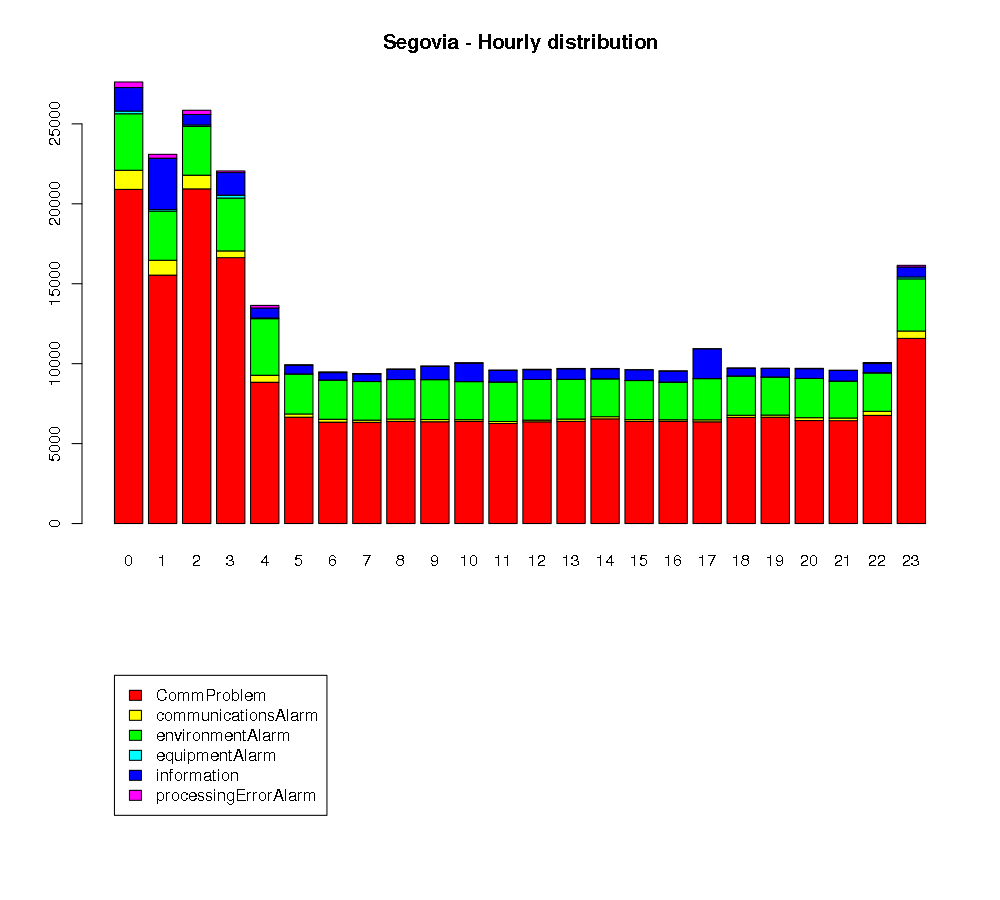
\includegraphics[width=\textwidth]{./img/segovia_timeline.png}
 \caption{Hourly distribution for Station C (stacked)} \label{fig:segovia_timeline}
\end{figure}
\begin{figure}[htb]
 \centering
 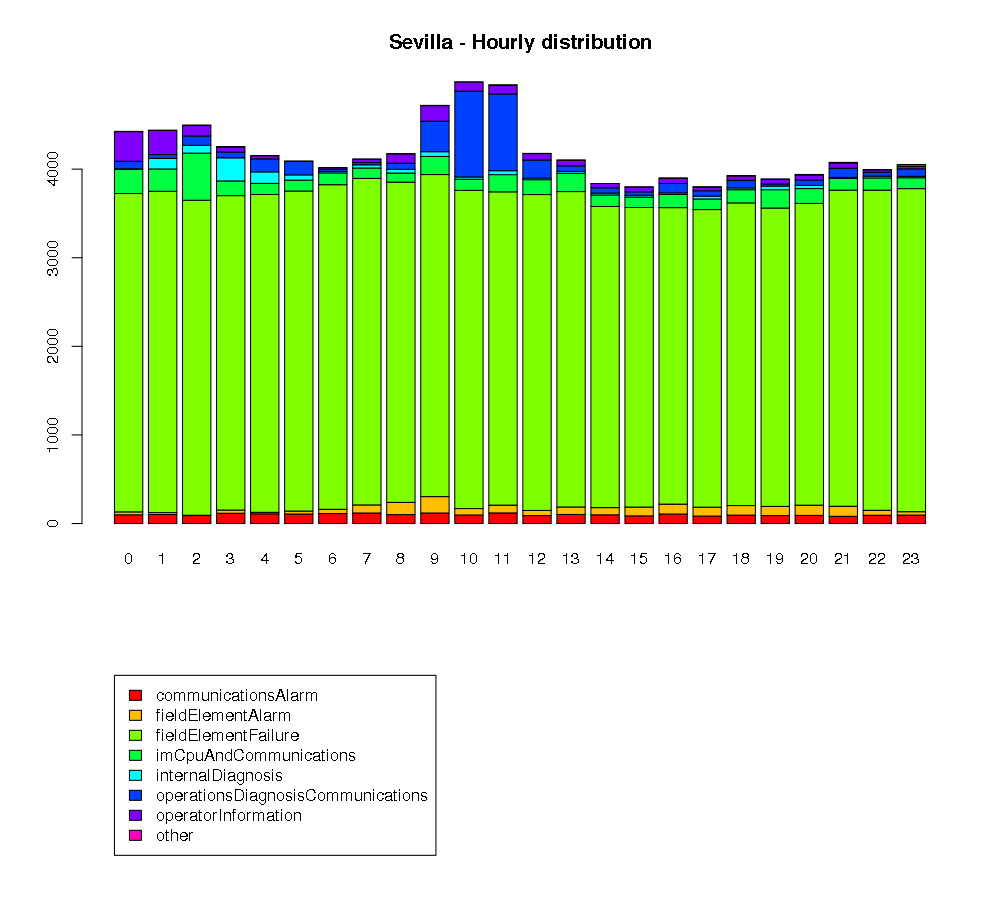
\includegraphics[width=\textwidth]{./img/sevilla_timeline.png}
 \caption{Hourly distribution for Station D (stacked)} \label{fig:sevilla_timeline}
\end{figure}

\clearpage

\section{Working methods}
\label{sec:methods}
For the development of this project, we have found a vast amount of useful tools and software which will provide an invaluable help in the different processes of our work. The main tool used will be the \emph{R} language\cite{ihaka1996r}, a very powerful tool commonly used for handling large amounts of data in an efficient way, and for which a vast amount of tools are available for our needs. R, and the IDE we are using, \emph{RStudio}\cite{racine2012rstudio} are open source software and available at no cost.

Due to licensing and compatibility issues, we are not able to use \emph{Microsoft SQL Server} databases to handle data. This is highly inconvenient as the data provided by Thales is in form of MS SQL backup files, which we needed to migrate to a compatible system of our choice: \emph{MySQL}. Given the tabular nature of the data, another solution based on plain text files would not be recommendable - although possible to handle with R - at least at the earliest stages until we analyse all the information and reduce the number of variables to export. In order to perform these migration tasks, a \emph{Windows} platform with \emph{Microsoft SQL Server Express} was required. Migration was successfully possible after slight modification of indexes and field definitions to fix compatibility issues. Once in MySQL format, we can query our data from RStudio without being limited to any kind of platform type or operative system, and will indeed perform further stages of the project under \emph{Unix} platforms.

Among all the available algorithms which can be useful for our project, we have chosen the \emph{cSPADE} algorithm\cite{zaki2001spade} as our starting point. It provides the most straight-away solution for the kind of problem we are approaching, as it considers temporal characteristics and allows us to set time constraints very easily. Other algorithms will be studied and applied at convenience, in order to complement cSPADE and find weak points which we could improve.

\begin{table}
\begin{tabularx}{\textwidth}{|X|l|X|}
\hline \headcell{Goal} & \headcell{Priority} & \headcell{Method} \\ 
\hline
\hline Perform a preliminary statistical analysis to set the project grounds & Compulsory & Statistical analysis with R \\ 
\hline Identify differences between maintenance stations & Compulsory & Statistical analysis with R \\ 
\hline Obtain rules to predict alarms using data of other alarms occurrence & Compulsory & Data Mining algorithms with R \\ 
\hline Obtain a Bayesian network to overview causal relations between alarms & Compulsory & Bayesian Networks with GeNIe/SMILE \\ 
\hline Validate and evaluate rule sets. Determine confidence of predictions & Compulsory & Cross-validation and confidence analysis with R \\ 
\hline Extract additional rules from Bayesian network for rule-form implementation & Desirable & GeNIE/SMILE \\ 
\hline Identify rule sets which can be applied to different station types & Desirable & Inter-station cross-validation with R \\ 
\hline Obtain rules to predict events using data of system and environment variables & Optional & Data Mining algorithms with R \\ 
\hline Identify which system or environment variables are more decisive for alarm prediction & Optional & Data Mining algorithms with R \\ 
\hline 

\end{tabularx} 
\caption{Summary of project goals and methods} \label{tab:objectives_methods}
\end{table}


\section{Final comments}
The most important thing before starting any other step, is to completely understand the context and scenario of our project. We do not need to fully know and understand the details on the procedures of railway maintenance, as the nature of the machinery performed reparations is not of significant relevance for the achievement of the defined objectives. In any case where we would need better understanding of system functioning - such as for identifying causal relations between failure events - we would need assistance from expert employees directly related with maintenance.

At this point, we have already treated all received data in order to be able to freely handle it without restrictions from any desired system. Required conversions have been performed and all data is already prepared to be loaded and used in R scripts.

We have also defined the learning objectives for the project, and set a ground to achieve them from an \emph{Knowledge Discovery in Databases} approach. Furthermore, we have made a first insight into \emph{Data Mining} techniques and performed a first analysis on their adequacy for our project. Initial tools have already been selected: cSPADE and GeNIe/SMILE.

In the next stage of Trainmining, we will need to make a deeper insight into the provided databases. The procedures which we have already defined (time discretion and definition of observation times) will have to be performed, selecting the exact variables among all of them which are registered for each alarm.